\section{eo\-Gen\-Continue$<$ EOT $>$ Class Template Reference}
\label{classeo_gen_continue}\index{eoGenContinue@{eoGenContinue}}
Generational continuator: continues until a number of generations is reached.  


{\tt \#include $<$eo\-Gen\-Continue.h$>$}

Inheritance diagram for eo\-Gen\-Continue$<$ EOT $>$::\begin{figure}[H]
\begin{center}
\leavevmode
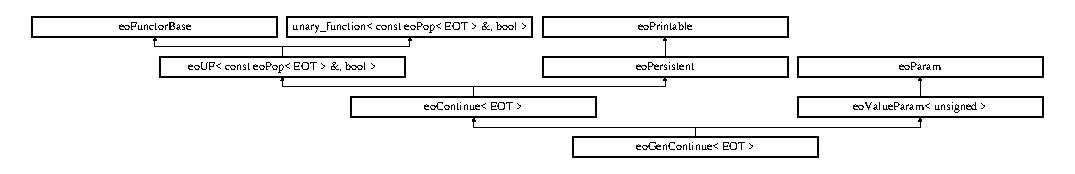
\includegraphics[height=1.89189cm]{classeo_gen_continue}
\end{center}
\end{figure}
\subsection*{Public Member Functions}
\begin{CompactItemize}
\item 
{\bf eo\-Gen\-Continue} (unsigned long \_\-total\-Gens)\label{classeo_gen_continue_a0}

\begin{CompactList}\small\item\em Ctor for setting a. \item\end{CompactList}\item 
{\bf eo\-Gen\-Continue} (unsigned long \_\-total\-Gens, unsigned long \&\_\-current\-Gen)\label{classeo_gen_continue_a1}

\begin{CompactList}\small\item\em Ctor for enabling the save/load the no. of generations counted. \item\end{CompactList}\item 
virtual bool {\bf operator()} (const {\bf eo\-Pop}$<$ {\bf EOT} $>$ \&\_\-v\-EO)\label{classeo_gen_continue_a2}

\begin{CompactList}\small\item\em Returns false when a certain number of generations is reached. \item\end{CompactList}\item 
virtual void {\bf total\-Generations} (unsigned long \_\-tg)\label{classeo_gen_continue_a3}

\begin{CompactList}\small\item\em Sets the number of generations to reach and sets the current generation to 0 (the begin). \item\end{CompactList}\item 
virtual unsigned long {\bf total\-Generations} ()\label{classeo_gen_continue_a4}

\begin{CompactList}\small\item\em Returns the number of generations to reach. \item\end{CompactList}\item 
virtual std::string {\bf class\-Name} (void) const \label{classeo_gen_continue_a5}

\item 
void {\bf read\-From} (std::istream \&\_\-\_\-is)
\begin{CompactList}\small\item\em Read object. \item\end{CompactList}\item 
void {\bf print\-On} (std::ostream \&\_\-\_\-os) const 
\begin{CompactList}\small\item\em Write object. \item\end{CompactList}\end{CompactItemize}
\subsection*{Public Attributes}
\begin{CompactItemize}
\item 
bool {\bf verbose}\label{classeo_gen_continue_o0}

\end{CompactItemize}
\subsection*{Private Attributes}
\begin{CompactItemize}
\item 
unsigned long {\bf rep\-Total\-Generations}\label{classeo_gen_continue_r0}

\item 
unsigned long {\bf this\-Generation\-Place\-Holder}\label{classeo_gen_continue_r1}

\item 
unsigned long \& {\bf this\-Generation}\label{classeo_gen_continue_r2}

\end{CompactItemize}


\subsection{Detailed Description}
\subsubsection*{template$<$class EOT$>$ class eo\-Gen\-Continue$<$ EOT $>$}

Generational continuator: continues until a number of generations is reached. 



Definition at line 34 of file eo\-Gen\-Continue.h.

\subsection{Member Function Documentation}
\index{eoGenContinue@{eo\-Gen\-Continue}!readFrom@{readFrom}}
\index{readFrom@{readFrom}!eoGenContinue@{eo\-Gen\-Continue}}
\subsubsection{\setlength{\rightskip}{0pt plus 5cm}template$<$class EOT$>$ void {\bf eo\-Gen\-Continue}$<$ {\bf EOT} $>$::read\-From (std::istream \& {\em \_\-\_\-is})\hspace{0.3cm}{\tt  [inline, virtual]}}\label{classeo_gen_continue_a6}


Read object. 

\begin{Desc}
\item[Parameters:]
\begin{description}
\item[{\em \_\-is}]A std::istream. \end{description}
\end{Desc}
\begin{Desc}
\item[Exceptions:]
\begin{description}
\item[{\em runtime\_\-std::exception}]If a valid object can't be read. \end{description}
\end{Desc}


Reimplemented from {\bf eo\-Continue$<$ EOT $>$} {\rm (p.\,\pageref{classeo_continue_a1})}.

Definition at line 83 of file eo\-Gen\-Continue.h.\index{eoGenContinue@{eo\-Gen\-Continue}!printOn@{printOn}}
\index{printOn@{printOn}!eoGenContinue@{eo\-Gen\-Continue}}
\subsubsection{\setlength{\rightskip}{0pt plus 5cm}template$<$class EOT$>$ void {\bf eo\-Gen\-Continue}$<$ {\bf EOT} $>$::print\-On (std::ostream \& {\em \_\-\_\-os}) const\hspace{0.3cm}{\tt  [inline, virtual]}}\label{classeo_gen_continue_a7}


Write object. 

It's called print\-On since it prints the object on a stream. \begin{Desc}
\item[Parameters:]
\begin{description}
\item[{\em \_\-os}]A std::ostream. \end{description}
\end{Desc}


Reimplemented from {\bf eo\-Continue$<$ EOT $>$} {\rm (p.\,\pageref{classeo_continue_a2})}.

Definition at line 88 of file eo\-Gen\-Continue.h.

The documentation for this class was generated from the following file:\begin{CompactItemize}
\item 
eo\-Gen\-Continue.h\end{CompactItemize}
